\chapter{Ambition, Fuel to Success}

This chapter follows Jim Rohn's lecture, as preserved in the curated LazyingArt LLC playlist, closely in narrative order. The surviving visual material does not preserve usable board work, so the mathematics here is a careful reconstruction of the lecture's process-logic rather than a transcription of chalkboard formulas. The lecture treats ambition as a structured dynamics: wish becomes desire, desire acquires discipline, dreams develop pull, service produces deserving, and small actions propagate through the rest of life.

\section{From Wish to Disciplined Eager Desire}

The lecture begins with a puzzle. Ambition is called a mystery, and then immediately reduced to a dictionary phrase: an eager desire for distinction, power, or fame. But the speaker does not leave the matter there. He first lingers over the ordinary word ``eager'' and notices that we use it freely for pleasures, parties, games, shopping, and social occasions, while we rarely speak of being eager for a better life, a better family, or greater prosperity. The point is not verbal. It is structural. A vague wish does not yet organize conduct.

\begin{definition}
In the logic of this lecture, ambition is not bare wanting. It is disciplined, eager desire: a desire strong enough to reorganize present action in the service of a future result.
\end{definition}

We can write the first schematic law of the chapter as
\begin{equation}
\text{ambition}=\text{disciplined, eager desire}.
\end{equation}
The lecture sharpens the contrast with a second relation:
\begin{equation}
\text{wish} \not\Rightarrow \text{change},
\qquad
\text{desire}+\text{discipline}\Rightarrow \text{change}.
\end{equation}
A wish names an outcome. Discipline binds that outcome to the present tense. If we want the meeting tomorrow to go well, we prepare today. If we want money later, we save now. If we want a better life later, we begin the work immediately.

A useful compression of the opening movement is
\begin{equation}
W \longrightarrow D \xrightarrow{\text{discipline}} A,
\end{equation}
where \(W\) is wish, \(D\) is desire, and \(A\) is ambition.

\begin{figure}
\centering
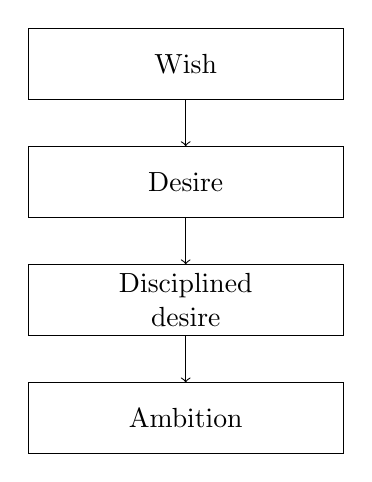
\begin{tikzpicture}[x=1cm,y=1cm]
\draw (0,0) rectangle (4,0.9);
\node at (2,0.45) {Wish};
\draw[->] (2,0) -- (2,-0.6);
\draw (0,-1.5) rectangle (4,-0.6);
\node at (2,-1.05) {Desire};
\draw[->] (2,-1.5) -- (2,-2.1);
\draw (0,-3.0) rectangle (4,-2.1);
\node[align=center] at (2,-2.55) {Disciplined\\ desire};
\draw[->] (2,-3.0) -- (2,-3.6);
\draw (0,-4.5) rectangle (4,-3.6);
\node at (2,-4.05) {Ambition};
\end{tikzpicture}
\end{figure}

The lecturer then makes the temporal character of ambition explicit:
\begin{equation}
\text{ambition}=\text{minute-by-minute, day-by-day mentality}.
\end{equation}
This matters. Ambition is not a single surge of feeling. It is a repeated alignment of today with tomorrow.

\subsection{Question \& Answer}

\paragraph{Question.} What turns a wish into ambition?

\paragraph{Answer.} Not intensity alone. The lecture's answer is that ambition appears when desire acquires backbone. A wish says, ``I would like the result.'' Ambition says, ``Because I want the result, I will change what I do now.'' The operative shift is from fantasy to present discipline.

\section{Dreams, Pull Power, and the Finished Future}

Once ambition has been defined inwardly, the lecture widens the frame. Why does one small group seem to build and enjoy fortune while a much larger group struggles merely to earn a living? The answer is not presented as sociology. It is presented as dream-power. Dreams are projections of the life we want to live, and they are not neutral pictures. They pull.

The lecture's next relations may be written as
\begin{equation}
\text{well-defined dream}\Rightarrow \text{pull power},
\qquad
\text{fuzzy future}\Rightarrow \text{little pull power}.
\end{equation}
Schematically,
\begin{equation}
\text{dream vividness}\uparrow \Rightarrow \text{motivational pull}\uparrow.
\end{equation}
This is the sense in which dreams ``drive'' and ``make us skip over obstacles.'' They do not remove the obstacle. They change the effective force exerted by the future upon the present. A vivid future pulls harder than a vague future.

The lecturer dramatizes this through pioneers crossing mountains and immigrants arriving with defined hopes. The image is exact: to move through hardship, one must see the far side before the body has reached it. In this sense the future is treated as finished in advance. One sees California while climbing the peak; one hears the cheers while still in the middle of the project.

We may compress the underlying logic as
\begin{equation}
\text{dreams} \Rightarrow \text{creative force stronger than obstacles}.
\end{equation}
The lecture does not mean that obstacles vanish. It means that the effective direction of motion is determined less by the push of hardship than by the pull of a sufficiently vivid end-state.

\subsection{Question \& Answer}

\paragraph{Question.} Why do well-defined dreams pull harder than obstacles push?

\paragraph{Answer.} Because definition gives the future shape. A fuzzy future cannot order present sacrifice. A vivid future can. Once the end is seen in advance, discomfort is no longer an isolated pain; it becomes part of a route. The obstacle remains, but its meaning changes.

\section{Franklin's Three Principles of Success}

After dreams and national examples, the lecture pivots to Ben Franklin and to practical laws of self-making. Franklin's value here is not antiquarian. He supplies a language for translating aspiration into repeated increments.

The first principle is that happiness does not arise from one large fragment of success, but from small advantages hammered out day by day. If we let \(a_n\) denote the \(n\)-th small advantage, then the lecture's process can be summarized by
\begin{align}
A_N &= \sum_{n=1}^{N} a_n,\\
a_n &= \text{a small advantage won on day }n.
\end{align}
This is not literal arithmetic. It is the compounding structure of the talk. Great achievement is not a single block handed to us at the end. It is an accumulation.

The second principle is Franklin's phrase that life is plastic. In the lecture this means
\begin{equation}
\text{life is plastic}\Rightarrow \text{self and environment are moldable}.
\end{equation}
A future form is first conceived, and then the shaping continues minute by minute, day by day, month by month, year by year. This principle links Franklin back to the lecture's earlier dream-image. The dream supplies the form; daily work supplies the molding.

The third principle is the most provocative:
\begin{equation}
\text{success}=\text{pleasure}.
\end{equation}
The point is not hedonism. It is that if our present activity is altogether empty, then even large external achievements will not amount to success in the full sense intended here. The lecture insists that one must be happy with what one has while pursuing what one wants. Big achievement does not excuse present deadness.

We may therefore restate Franklin's three claims in the lecture's own process-language:
\begin{align}
\text{big achievement} &= \sum \text{small advantages},\\
\text{life is plastic} &\Rightarrow \text{it can be shaped},\\
\text{success} &= \text{pleasure along the way}.
\end{align}

\section{William James and the Word ``Until''}

Franklin provides practical wisdom; William James provides the chapter's cleanest formal decomposition. The lecture introduces pragmatism as a habit of asking what an idea does, what use it has, and what practical results follow from it. Then James's answer to the question of success is given in two parts:
\begin{align}
S &= I + O,\\
I &= \text{inner ideal followed persistently with courage},\\
O &= \text{outer achievement related to that ideal}.
\end{align}
The lecture immediately ranks these two terms:
\begin{equation}
I \succ O.
\end{equation}
The first term is more important than the second. The inner ideal is primary because without it the outward term never stabilizes into genuine success. This yields a simple schematic consequence:
\begin{align}
I=0 &\Rightarrow S \text{ collapses in the strong sense},\\
I>0,\ O=0 &\Rightarrow S \text{ remains possible and already begins},\\
I>0,\ O>0 &\Rightarrow S \text{ is success in both inward and outward form}.
\end{align}
Again, this is a transcript-backed reconstruction, not a board equation, but it captures the logic of the lecture very closely.

The operative word in this section is ``until.'' Read until the skill changes. Attend until the matter makes sense. Practice until it is right. Continue until one learns, changes, and grows. The lecture's iterative law is
\begin{equation}
\text{do it until} \Rightarrow \text{learn, change, grow}.
\end{equation}
Or, in a more expanded form,
\begin{equation}
\text{step by step}+\text{piece by piece}+\text{book by book}+\text{seminar by seminar}
\Rightarrow
\text{progress}.
\end{equation}
The power of ``until'' is that it converts duration from an objection into an operator. Time no longer measures delay; it measures persistence.

\subsection{Question \& Answer}

\paragraph{Question.} How can one already count as successful before the outer achievement is complete?

\paragraph{Answer.} Because the lecture refuses to identify success with the last trophy alone. If the inner ideal is alive, and if it is being pursued persistently with courage, then success is already active in the present. The outer result matters, but the first term governs the meaning of the second.

\section{Small Changes and the Social Field of Success}

The lecture now returns from philosophers to the everyday visible signs of inward change. What does success look like before any large public result appears? The answer is: it first appears in little things. We change sleep, mood, greeting, attention, and family presence, and then these seemingly local corrections begin to alter the rest of the field.

The simplest form of the rule is
\begin{equation}
\text{change within} \Rightarrow \text{change around}.
\end{equation}
A companion relation is
\begin{equation}
\text{respond differently to life} \Rightarrow \text{life responds differently to you}.
\end{equation}
This is still the lecture's same structure. A local shift reorganizes a larger system.

\paragraph{Worked example.} The lecture's example of getting up earlier can be written as a narrow causal chain:
\begin{align}
d_1 &= \text{go to bed a little earlier},\\
d_2 &= \text{rise in a better mood},\\
d_3 &= \text{begin the day more effectively},\\
d_4 &= \text{work with other people more gracefully}.
\end{align}
Thus
\begin{equation}
d_1 \Rightarrow d_2 \Rightarrow d_3 \Rightarrow d_4.
\end{equation}
What is important is not the specific habit. It is the lecture's insistence that the first small correction can propagate.

The same logic governs the little courtesies the speaker recommends: smile at someone in traffic, greet the front desk, embrace the family before collapsing on the sofa. These are not ornamental moral decorations. They are early visible evidence that a person has begun to take charge of his own interior state.

The section then broadens into a social theorem of sorts:
\begin{equation}
\text{each of us needs all of us}.
\end{equation}
This is the lecture's denial that success is solitary. Even the person who appears to work alone is supported by toleration, service, patience, and prior contributions from others. Thus gratitude is not merely polite. It is a truthful accounting of the real architecture of action.

\section{Ambition, Not Greed}

After the lecture has built ambition from desire, dreams, daily progress, and social dependence, it returns to the word itself and defines it against its corrupt doubles. Joseph Epstein's phrase is the bridge:
\begin{equation}
\text{ambition}=\text{fuel of achievement}.
\end{equation}
But the lecture immediately adds a warning. Ambition is not greed. It is not avarice. It is not victory at another person's expense:
\begin{equation}
\text{ambition}\neq \text{greed},
\qquad
\text{ambition}\neq \text{avarice}.
\end{equation}

The distinction is sharpened through a useful pair:
\begin{equation}
\text{desire}=\text{what you want},
\qquad
\text{ambition}=\text{how you get there}.
\end{equation}
Desire by itself can be healthy or unhealthy. It can want the tallest building in town. But the lecturer then offers two ways of satisfying that desire. One way is destructive: tear the other buildings down. The other way is constructive: see the taller building, plan it, gather the team, endure the weather, and build it.

We can summarize the contrast by
\begin{equation}
\text{destructive desire}\Rightarrow \text{tear others down},
\qquad
\text{constructive ambition}\Rightarrow \text{build upward}.
\end{equation}
The Judas example serves exactly this purpose. Wealth acquired through betrayal does not count as ambition because the process deforms the person. The lecture is therefore not measuring outcomes alone. It is measuring what one becomes in pursuit of them.

\subsection{Question \& Answer}

\paragraph{Question.} How is ambition different from greed if both seem to want more?

\paragraph{Answer.} Greed wants gain without regard for the damage done to others or to the self. Ambition, as the lecture defines it, accepts the discipline of construction. It builds, serves, plans, endures, and expresses something positive. The difference lies not merely in the amount desired, but in the method and the moral geometry of the pursuit.

\section{Enlightened Self-Interest, Deserving, and the Network of Disciplines}

The last major movement of the lecture gathers the previous threads into a more operational system. Self-interest, we are told, is not itself a defect. The defect begins when self-interest is left unenlightened. The lecture's law is
\begin{equation}
\text{enlightened self-interest}\Rightarrow \text{benefit by service to others},
\end{equation}
whereas
\begin{equation}
\text{self-interest at the expense of others}\Rightarrow \text{greed / evil}.
\end{equation}
This yields the lecture's sharp contrast:
\begin{equation}
\text{enlightened self-interest}\Rightarrow \text{wealth},
\qquad
\text{self-preservation alone}\Rightarrow \text{poverty}.
\end{equation}
The story of the man who, while broke and living in a hotel, still spends hours helping feed the homeless is not a sentimental aside. It is an instance of the lecture's causal claim that service changes the social world that later changes us.

From here the lecture passes to giving and investment:
\begin{equation}
\text{if you wish to receive, you must give},
\end{equation}
\begin{equation}
\text{giving}=\text{investment},
\qquad
\text{investment}\Rightarrow \text{return multiplied}.
\end{equation}
This is why the maxim ``do more than you get paid for'' appears here. It is not merely moral advice. It is an investment rule:
\begin{equation}
\text{do more than you get paid for} \Rightarrow \text{investment in future return}.
\end{equation}
So too with sales:
\begin{equation}
\text{make a sale} \Rightarrow \text{make a living},
\qquad
\text{serve beyond the sale} \Rightarrow \text{make a fortune}.
\end{equation}

The lecture then states one of its cleanest laws:
\begin{equation}
\text{life responds to deserve, not need}.
\end{equation}
The false law is rejected:
\begin{equation}
\text{need} \not\Rightarrow \text{reap}.
\end{equation}
The operative law is planting:
\begin{equation}
\text{plant} \Rightarrow \text{reap}.
\end{equation}
The soil metaphor is exact. Need does not move the soil. Seed does. Therefore the lecture expands seed into a bundle of practical inputs:
\begin{equation}
\text{seed}+\text{effort}+\text{discipline}+\text{service}\Rightarrow \text{return}.
\end{equation}
What appears as a moral maxim is also a process rule: bring the field something to work with.

The same structure governs searching:
\begin{equation}
\text{search} \Rightarrow \text{find},
\qquad
\text{searching} \Rightarrow \{\text{ideas},\text{inspiration},\text{hope},\text{contacts}\}.
\end{equation}
The lecture's point is not mystical. If we want to find, we must enter the places where finding can occur: seminar, library, bookstore, class, training.

Finally, the lecture closes with a systems-claim about discipline itself:
\begin{equation}
\text{one discipline affects another},
\qquad
\text{all disciplines affect each other}.
\end{equation}
In its broadest form,
\begin{equation}
\text{everything affects everything else}.
\end{equation}
This gives both a negative and a positive cascade:
\begin{align}
\text{every letdown} &\Rightarrow \text{affects the rest},\\
\text{every new discipline} &\Rightarrow \text{affects the rest}.
\end{align}

\begin{figure}
\centering
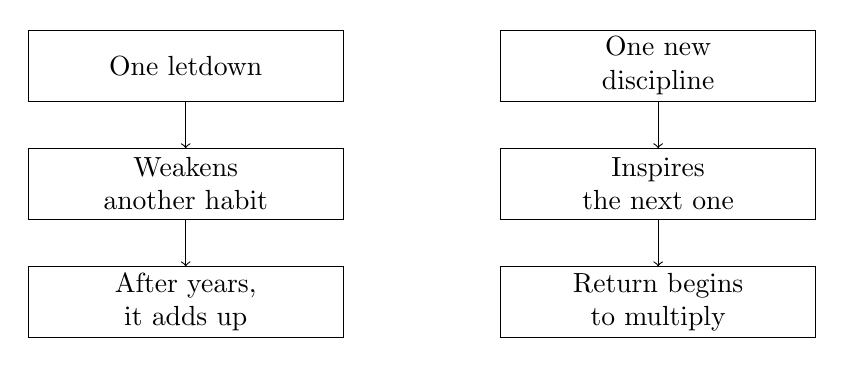
\begin{tikzpicture}[x=1cm,y=1cm]
\draw (0,0) rectangle (4,0.9);
\node[align=center] at (2,0.45) {One letdown};
\draw[->] (2,0) -- (2,-0.6);
\draw (0,-1.5) rectangle (4,-0.6);
\node[align=center] at (2,-1.05) {Weakens\\ another habit};
\draw[->] (2,-1.5) -- (2,-2.1);
\draw (0,-3.0) rectangle (4,-2.1);
\node[align=center] at (2,-2.55) {After years,\\ it adds up};

\draw (6,0) rectangle (10,0.9);
\node[align=center] at (8,0.45) {One new\\ discipline};
\draw[->] (8,0) -- (8,-0.6);
\draw (6,-1.5) rectangle (10,-0.6);
\node[align=center] at (8,-1.05) {Inspires\\ the next one};
\draw[->] (8,-1.5) -- (8,-2.1);
\draw (6,-3.0) rectangle (10,-2.1);
\node[align=center] at (8,-2.55) {Return begins\\ to multiply};
\end{tikzpicture}
\end{figure}

\paragraph{Worked example.} The lecture gives an explicit positive cascade:
\begin{align}
c_1 &= \text{walk around the block},\\
c_2 &= \text{eat right},\\
c_3 &= \text{buy a book},\\
c_4 &= \text{keep a journal},\\
c_5 &= \text{develop skills}.
\end{align}
Hence
\begin{equation}
c_1 \Rightarrow c_2 \Rightarrow c_3 \Rightarrow c_4 \Rightarrow c_5.
\end{equation}
This is why the lecture insists on the smallest action:
\begin{equation}
\text{smallest action} \Rightarrow \text{momentum}.
\end{equation}
And once action has begun,
\begin{equation}
\text{accomplishment} \Rightarrow \text{inspiration for the next accomplishment}.
\end{equation}
This is the chapter's final mathematical image: not one dramatic leap, but a compounding process in which local disciplines alter neighboring disciplines.

\subsection{Question \& Answer}

\paragraph{Question.} Why does life respond to deserve rather than need?

\paragraph{Answer.} Because the lecture treats life as a field rather than as a pitying judge. A field does not answer complaint; it answers seed. Need names absence. Deserving, in this lecture, names what has actually been planted into the world: effort, service, willingness, and disciplined action.

\subsection{Question \& Answer}

\paragraph{Question.} How can the least action matter if the problems are large?

\paragraph{Answer.} Because disciplines are coupled. A single action is not isolated. It changes mood, schedule, attention, competence, and the probability of the next action. The smallest action matters precisely because it is not the last action; it is the first one in a cascade.

\section{Summary}

We can now see the full architecture of the lecture. Ambition begins as disciplined, eager desire and immediately acquires a temporal form: today must be altered for tomorrow to change. Dreams then supply pull, especially when the future is well defined and vividly seen in advance. Franklin translates ambition into small daily advantages, moldability, and pleasure in the process. James decomposes success into an inner ideal and an outer achievement, while insisting on the primacy of the first term and on the discipline of ``until.'' The lecture then returns to everyday evidence, showing that inner reform first appears in little habits and in better relations with other people. Finally, ambition is rescued from greed, self-interest is enlightened by service, deserving replaces mere need, and the chapter ends with a strong systems-claim: disciplines affect one another. In this sense the lecture's deepest mathematical image is one of compounding structure. A life changes because one disciplined act becomes the condition of the next.